%%%%%%%%%%%%%%%%%%%%%%%%%%%%%%%%%%%%%%%%%
% Jacobs Landscape Poster
% LaTeX Template
% Version 1.1 (14/06/14)
%
% Created by:
% Computational Physics and Biophysics Group, Jacobs University
% https://teamwork.jacobs-university.de:8443/confluence/display/CoPandBiG/LaTeX+Poster
% 
% Further modified by:
% Nathaniel Johnston (nathaniel@njohnston.ca)
%
% This template has been downloaded from:
% http://www.LaTeXTemplates.com
%
% License:
% CC BY-NC-SA 3.0 (http://creativecommons.org/licenses/by-nc-sa/3.0/)
%
%%%%%%%%%%%%%%%%%%%%%%%%%%%%%%%%%%%%%%%%%

%----------------------------------------------------------------------------------------
%	PACKAGES AND OTHER DOCUMENT CONFIGURATIONS
%----------------------------------------------------------------------------------------

\documentclass[final]{beamer}

\usepackage{algorithm}
\usepackage{algorithmic}
\usepackage{etoolbox}
\AtBeginEnvironment{algorithm}{%
  \setlength{\columnwidth}{\linewidth}%
}

\usepackage[scale=1.24]{beamerposter} % Use the beamerposter package for laying out the poster
\usepackage{tipa}
\usepackage{amsmath}
\usepackage{amssymb}
\usepackage{amsfonts}
\usetheme{confposter} % Use the confposter theme supplied with this template
\usepackage{sidecap}
\setbeamercolor{block title}{fg=ngreen,bg=white} % Colors of the block titles
\setbeamercolor{block body}{fg=black,bg=white} % Colors of the body of blocks
\setbeamercolor{block alerted title}{fg=white,bg=dblue!70} % Colors of the highlighted block titles
\setbeamercolor{block alerted body}{fg=black,bg=dblue!10} % Colors of the body of highlighted blocks
% Many more colors are available for use in beamerthemeconfposter.sty

%-----------------------------------------------------------
% Define the column widths and overall poster size
% To set effective sepwid, onecolwid and twocolwid values, first choose how many columns you want and how much separation you want between columns
% In this template, the separation width chosen is 0.024 of the paper width and a 4-column layout
% onecolwid should therefore be (1-(# of columns+1)*sepwid)/# of columns e.g. (1-(4+1)*0.024)/4 = 0.22
% Set twocolwid to be (2*onecolwid)+sepwid = 0.464
% Set threecolwid to be (3*onecolwid)+2*sepwid = 0.708

\newlength{\sepwid}
\newlength{\onecolwid}
\newlength{\twocolwid}
\newlength{\threecolwid}
\setlength{\paperwidth}{72in} % A0 width: 46.8in
\setlength{\paperheight}{48in} % A0 height: 33.1in
\setlength{\sepwid}{0.024\paperwidth} % Separation width (white space) between columns
\setlength{\onecolwid}{0.22\paperwidth} % Width of one column
\setlength{\twocolwid}{0.464\paperwidth} % Width of two columns
\setlength{\threecolwid}{0.708\paperwidth} % Width of three columns
\setlength{\topmargin}{-0.5in} % Reduce the top margin size
%-----------------------------------------------------------

\usepackage{etoolbox}
\makeatletter
\patchcmd{\beamer@@tmpl@headline}{wd=47in}{wd=71in}{}{}
\makeatother

\usepackage{graphicx}  % Required for including images
\usepackage{verbatim}
\usepackage{booktabs} % Top and bottom rules for tables

\usepackage{wrapfig}

%----------------------------------------------------------------------------------------
%	TITLE SECTION 
%----------------------------------------------------------------------------------------
\usepackage{stmaryrd}
\newcommand{\tuple}[1]{\ensuremath{\left \langle #1\right \rangle}}
\newcommand{\sem}[1]{[\mkern-6mu[#1]\mkern-6mu]} %\newcommand{\sem}[1]{\llbracket #1\rrbracket}

\usetikzlibrary{trees}
\usetikzlibrary{fit}
\usetikzlibrary{calc}
\usetikzlibrary{bayesnet}

\usepackage[normalem]{ulem}

\newcommand{\theSystem}{\textsc{ProgramSample}}
\title{Sampling for Bayesian Program Learning} % Poster title


\author{Kevin Ellis, Armando Solar-Lezama, and Joshua B. Tenenbaum} % Author(s)

\institute{Massachusetts Institute of Technology} % Institution(s)

%----------------------------------------------------------------------------------------

\begin{document}
\addtobeamertemplate{headline}{} 
{\begin{tikzpicture}[remember picture, overlay]
     \node [anchor=north east, inner sep=3cm]  at (current page.north east)
           {
\includegraphics[height=7cm]{csail.png}};
                \node [anchor=north west, inner sep=3cm]  at (current page.north west)
     {
\includegraphics[height=5cm]{bcs.png}};
\end{tikzpicture}}

\addtobeamertemplate{block end}{}{\vspace*{2ex}} % White space under blocks
\addtobeamertemplate{block alerted end}{}{\vspace*{2ex}} % White space under highlighted (alert) blocks

\setlength{\belowcaptionskip}{2ex} % White space under figures
\setlength\belowdisplayshortskip{2ex} % White space under equations

\begin{frame}[t] % The whole poster is enclosed in one beamer frame

\begin{columns}[t] % The whole poster consists of three major columns, the second of which is split into two columns twice - the [t] option aligns each column's content to the top

\begin{column}{\sepwid}\end{column} % Empty spacer column

\begin{column}{\onecolwid} % The first column

%----------------------------------------------------------------------------------------
%	OBJECTIVES
%----------------------------------------------------------------------------------------


\begin{alertblock}{Problem statement}
  \textbf{Bayesian Program Learning:} Learn programs from input/output examples, framed as Bayesian inference.
  Given a prior over programs, condition on examples. 
  In this work we approximate the posterior by a set of samples.

  \begin{itemize}
  \item \textbf{Efficient in practice}: synthesizes non-trivial programs in minutes
  \item \textbf{Theoretical guarantees}: our algorithm, \theSystem , generates iid samples from a distribution that provably approximates the true posterior 
    \end{itemize}

Sampling text edit programs:
  
\centering\begin{tikzpicture}
\node[draw,rounded corners](problem)
     {\begin{tabular}{lr}
      Input & Output \\\hline
      ``1/21/2001'' & ``01''
     \end{tabular}};
\node[draw,rounded corners](sampledPrograms) at (0,-7)
     {\begin{tabular}{lr}
         A sampled program & English interpretation\\\hline
         {\ttfamily\small \hspace{-\mylength}substr(pos('0',-1),-1)} & ``last 0 til end'' \\
      {\ttfamily\small \hspace{-\mylength}const('01')}       & ``output 01''\\
      {\ttfamily\small \hspace{-\mylength}substr(-2,-1)} & ``take last two''
     \end{tabular}};
\draw[->,thick](problem.south) -- (sampledPrograms.north);
\end{tikzpicture}
\end{alertblock}

%----------------------------------------------------------------------------------------
%	INTRODUCTION
%----------------------------------------------------------------------------------------

\begin{block}{Two Key Ingredients}
  How can we get both practical  performance and theoretical guarantees for a problem that feels so obviously intractable? Combine two ideas:
  \begin{itemize}
  \item \textbf{Sketching:} The program's high-level structure is
    already given as a \emph{sketch}, like a recursive grammar over
    expressions. Consider \emph{finite} programs (bounded size, bounded
    runtime, bounded memory consumption), which can be modeled in a
    constraint solver: this does the heavy lifting of searching for programs. Here we use a SAT solver.
  \item \textbf{Sampling via random XOR constraints:} Once a program learning problem has been converted to SAT,
    we can sample programs (SAT solutions) by adding random XOR constraints to the SAT formula,
    an idea first introduced in Gomes et al 2006.
  \end{itemize}
\end{block}

%------------------------------------------------

\begin{block}{Problem Framing}
  \begin{itemize}
  \item Sketch specifies a large but finite set of programs, $S$
  \item Program description length: $\lvert x \rvert$ for $x\in S$
  \item Prior over programs: $\propto 2^{- \lvert x \rvert }$
  \item Posterior over programs: call this $p(x)$, defined as $\propto 2^{- \lvert x \rvert } \mathds{1}[x \text{ consistent with input/output examples}]$
  \end{itemize}
  Our goal then  is to sample from $p(\cdot)$.
\end{block}

%----------------------------------------------------------------------------------------

\end{column} % End of the first column

\begin{column}{\sepwid}\end{column} % Empty spacer column

\begin{column}{\twocolwid} % Begin a column which is two columns wide (column 2)

\begin{columns}[t,totalwidth=\twocolwid] % Split up the two columns wide column

\begin{column}{\onecolwid}\vspace{-.6in} % The first column within column 2 (column 2.1)

%----------------------------------------------------------------------------------------
%	MATERIALS
%----------------------------------------------------------------------------------------


  \begin{block}{Background: Program Synthesis by SAT Solving}

\hspace{-2.5cm}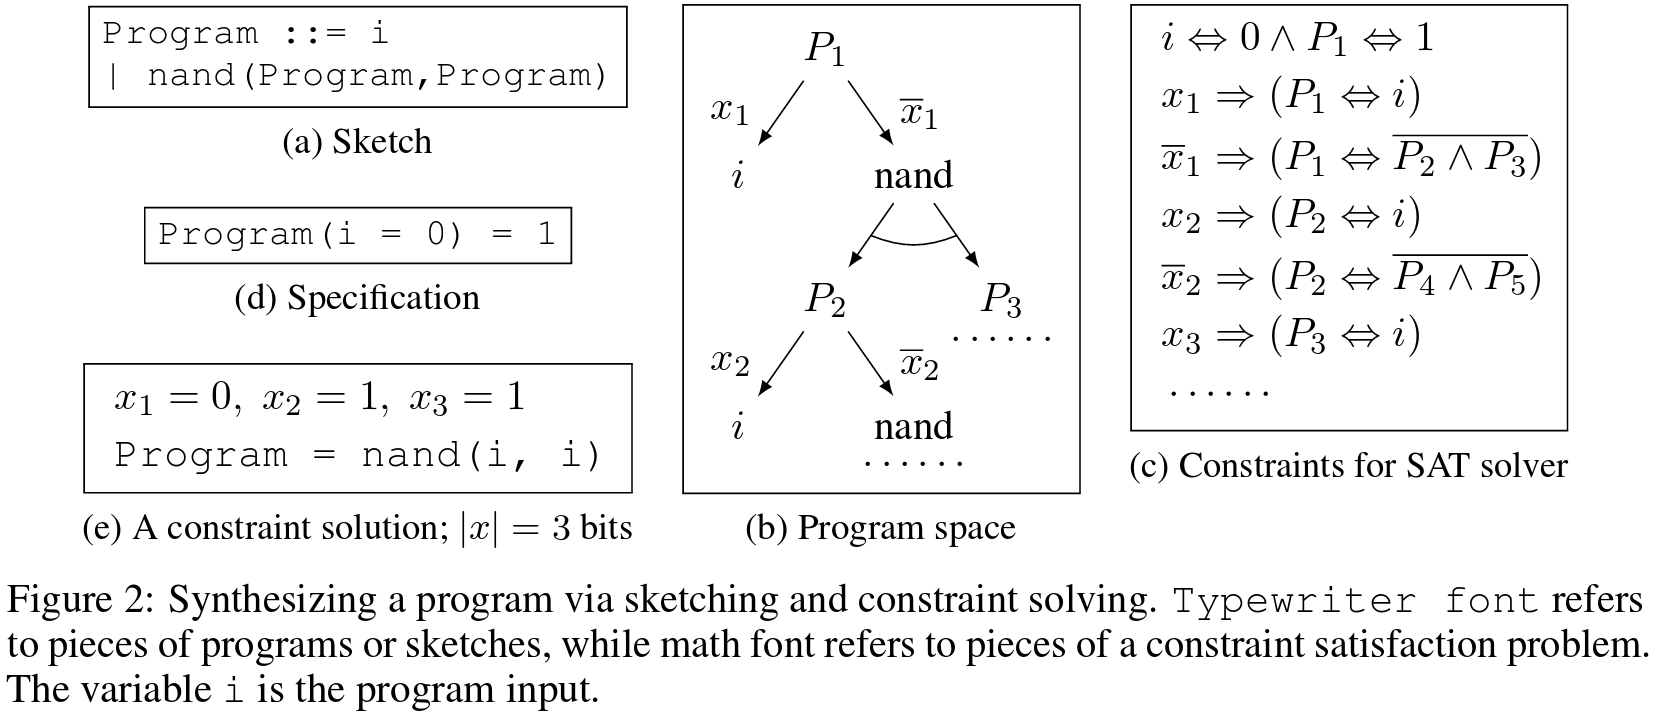
\includegraphics[width=45cm]{background.png}
  \end{block}

    \begin{block}{Sampling by Random XOR Constraints}
Embed $X$ within a larger set $E$ where sampling uniformly from $E$ samples from $  q(x) \propto     2^{-\text{min}(\lvert x \rvert,d) }$, where $d$ bounds the tilt of $q(\cdot)$:
  \begin{equation}
    E = \{(x,y) \text{ }:\text{ } x\in X,  \bigwedge_{1\leq j \leq d} \lvert x \rvert \geq j\Rightarrow y_j=1 \}
  \end{equation}
  Sample approximately uniformly from $E$ by fixing the parity of random sums (XOR's) of SAT variables. Use $K$ such sums. \# satisfying members of $E$ is $\approx 2^{-K}|E|$. Accept sample w.p. $A(x) = \min (1,2^{-|x| + d})$ to correct for $q(\cdot)$.

\vspace{0.9cm}
  \begin{tabular}{cl}
    \begin{tabular}{c}
      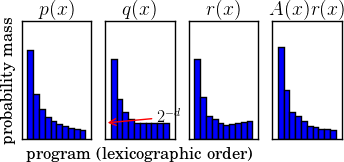
\includegraphics[width=25cm]{cartoon_small.png} 
    \end{tabular}&
    \begin{tabular}{l}
      \parbox{15cm}{\emph{Summary}: Approximate $p(x)$ by $q(x)$, embed in $E$, approximately uniform samples of $E$ give $r(x)$, distribution of samples is $\propto A(x)r(x)$}
      \end{tabular}
    \end{tabular}

    \end{block}
    
\begin{block}{Pseudocode: Outer optimization loop}

Minimize Eq.~\ref{descriptionLength} with an SMT solver in an inner loop:
\begin{algorithm}[H] %[tb]
   \label{optimization}
\begin{algorithmic}
  \STATE {\bfseries function UnsupervisedProgramSynthesis:}
   \STATE {\bfseries Input:} Grammar $\mathcal{G}$, grammar start symbol $P$, denotation $\sem{\cdot}$, observations $\{x_i\}_{i = 1}^N$, noise model, prior over program input 
   \STATE {\bfseries Output:} Program $f$, $N$ program inputs, description length $\ell$
   \STATE // $I_i$ is an (unknown) program input the SMT solver will find
   \STATE // Fresh variables unused in any existing formula
   \STATE $I_1,I_2,\cdots,I_N = ${\bfseries FreshInputVariable()}
   \STATE // Define hypothesis space and model program executions
   \STATE // $l_f = $ program description length, $A = $ set of SMT constraints
   \STATE $l_f,\{z_i\}_{i = 1}^N,A\leftarrow${\bfseries SMTEncoding}($\mathcal{G}, \sem{\cdot}, P,\{I_i\}_{i = 1}^N$)
   \STATE // Compute total description length $\ell$
   \STATE $\ell = ${\bfseries FreshRealVariable()}
   \STATE $A\leftarrow A\cup \{\ell = l_f - \sum_i ( \log P(x_i|z_i) +  \log P(I_i) \}$
   \WHILE{$A$ satisfiable according to SMT solver}
   \STATE $\sigma\leftarrow \text{ a satisfying solution to }A$
   \STATE $A\leftarrow A\cup \{ \ell < \sigma [\ell] \}$
   \ENDWHILE
   \STATE {\bfseries let} $f = \text{ unique program in $\mathcal{G}$ specified by $\sigma$}$
   \STATE {\bfseries return} $f,\{\sigma[I_i]\}_{i = 1}^N,\sigma[\ell]$
\end{algorithmic}
\end{algorithm}
\end{block}

%\begin{block}{SMT Encoding}

  
%  \end{block}

%----------------------------------------------------------------------------------------

\end{column} % End of column 2.1

\begin{column}{\onecolwid}\vspace{-.6in} % The second column within column 2 (column 2.2)

%----------------------------------------------------------------------------------------
%	METHODS
%----------------------------------------------------------------------------------------

\begin{block}{Domain: Visual concepts}
  Humans can quickly learn many abstract visual concepts, often from few examples. 
  Pairs of examples of twelve SVRT~\cite{fleuret2011comparing} concepts:

    \vspace{0.5cm}
%  \begin{figure}[h]\centering
%  \begin{minipage}[b]{10cm}\centering
    \begin{tikzpicture}\centering
      \node at (13,8) {\uline{Concepts 1--6}};
      \node [rotate = 90] at (-4,3) {\uline{Examples}};
\node[draw,inner sep=1pt] at (27.5,0)
{\includegraphics[width=4.5cm]{svrt/results_problem_8/sample_1_0009.png}};
\node[draw,inner sep=1pt] at (27.5,4.5)
{\includegraphics[width=4.5cm]{svrt/results_problem_8/sample_1_0051.png}};
\node[draw,inner sep=1pt] at (22,0)
{\includegraphics[width=4.5cm]{svrt/results_problem_20/sample_1_0009.png}};
\node[draw,inner sep=1pt] at (22,4.5)
{\includegraphics[width=4.5cm]{svrt/results_problem_20/sample_1_0051.png}};
\node[draw,inner sep=1pt] at (16.5,0)
{\includegraphics[width=4.5cm]{svrt/results_problem_10/sample_1_0009.png}};
\node[draw,inner sep=1pt] at (16.5,4.5)
{\includegraphics[width=4.5cm]{svrt/results_problem_10/sample_1_0051.png}};
\node[draw,inner sep=1pt] at (11,0)
{\includegraphics[width=4.5cm]{results_problem_16/sample_1_0009.png}};
\node[draw,inner sep=1pt] at (11,4.5)
{\includegraphics[width=4.5cm]{results_problem_16/sample_1_0051.png}};
\node[draw,inner sep=1pt] at (5.5,0)
{\includegraphics[width=4.5cm]{results_problem_3/sample_1_0009.png}};
\node[draw,inner sep=1pt] at (5.5,4.5)
{\includegraphics[width=4.5cm]{results_problem_3/sample_1_0051.png}};
\node[draw,inner sep=1pt] at (0,0)
{\includegraphics[width=4.5cm]{results_problem_9/sample_1_0010.png}};
\node[draw,inner sep=1pt] at (0,4.5)
{\includegraphics[width=4.5cm]{results_problem_9/sample_1_0011.png}};
\end{tikzpicture}
%\caption{Left: Pairs of examples of three SVRT concepts taken from \cite{fleuret2011comparing}. Right: the program we synthesize from the leftmost pair. This is a turtle program capable of drawing this pair of pictures and is parameterized by a set of latent variables: shape, distance, scale, initial position, initial orientation.}
%\label{fig:squares}
%\end{figure}

    \vspace{0.5cm}
%  \begin{figure}[h]\centering
%  \begin{minipage}[b]{10cm}\centering
    \begin{tikzpicture}\centering
      \node at (13,8) {\uline{Concepts 7--12}};
      \node [rotate = 90] at (-4,3) {\uline{Examples}};
\node[draw,inner sep=1pt] at (27.5,0)
{\includegraphics[width=4.5cm]{svrt/program_induction_data/results_problem_18/sample_0_0009.png}};
\node[draw,inner sep=1pt] at (27.5,4.5)
{\includegraphics[width=4.5cm]{svrt/program_induction_data/results_problem_18/sample_0_0051.png}};
\node[draw,inner sep=1pt] at (22,0)
{\includegraphics[width=4.5cm]{svrt/program_induction_data/results_problem_21/sample_1_0009.png}};
\node[draw,inner sep=1pt] at (22,4.5)
{\includegraphics[width=4.5cm]{svrt/program_induction_data/results_problem_21/sample_1_0051.png}};
\node[draw,inner sep=1pt] at (16.5,0)
{\includegraphics[width=4.5cm]{svrt/program_induction_data/results_problem_22/sample_1_0009.png}};
\node[draw,inner sep=1pt] at (16.5,4.5)
{\includegraphics[width=4.5cm]{svrt/program_induction_data/results_problem_22/sample_1_0051.png}};
\node[draw,inner sep=1pt] at (11,0)
{\includegraphics[width=4.5cm]{svrt/program_induction_data/results_problem_16/sample_0_0009.png}};
\node[draw,inner sep=1pt] at (11,4.5)
{\includegraphics[width=4.5cm]{svrt/program_induction_data/results_problem_16/sample_0_0051.png}};
\node[draw,inner sep=1pt] at (5.5,0)
{\includegraphics[width=4.5cm]{svrt/program_induction_data/results_problem_7/sample_1_0009.png}};
\node[draw,inner sep=1pt] at (5.5,4.5)
{\includegraphics[width=4.5cm]{svrt/program_induction_data/results_problem_7/sample_1_0051.png}};
\node[draw,inner sep=1pt] at (0,0)
{\includegraphics[width=4.5cm]{svrt/program_induction_data/results_problem_6/sample_1_0010.png}};
\node[draw,inner sep=1pt] at (0,4.5)
{\includegraphics[width=4.5cm]{svrt/program_induction_data/results_problem_6/sample_1_0011.png}};
\end{tikzpicture}
    
  Our system learns SVRT concepts by
 synthesizing a program that
  can draw example images within that concept. Learning occurs not from pixel-level input,
  but from the output of an image parser:

    \vspace{0.5cm}\begin{tikzpicture}
    \node[draw,rounded corners](original) at (-1,0)
         {\includegraphics[width=5cm]{unparsed.png}};
         \node[draw,rounded corners](segmented) at (8,0)
              {\includegraphics[width=5cm]{segmented.png}};
              \draw[->,ultra thick](original.east) -- (segmented.west);
              \node[draw,rounded corners](parsed) at (22,0)
                   {\begin{aligned}
                       &s_1 = \mbox{Shape}(\mbox{id} = 1,\mbox{scale} = 1,\\
                       &\hspace{6.5cm}x = 10,y = 15)\\
                       &s_2 = \mbox{Shape}(\mbox{id} = 2,\mbox{scale} = 1,\\
                       &\hspace{6.5cm}x = 27,y = 54)\\
                       &\mbox{borders}(s_1,s_2)
                   \end{aligned}};
                   \draw[->,ultra thick](segmented.east) -- (parsed.west);
  \end{tikzpicture}

%\if false
    Program representation:
    \begin{itemize}
    \item Program inputs: shapes, coordinates, distances, angles, scales
      \item Program output: Image parse
      \item Constraints on program space: control a turtle, but...
        \begin{itemize}
        \item Restricted to alternatingly moving and drawning
        \item No arithmetic on real variables
        \item No rotation of shapes
          %Movement: change coordinate/orientation, rotate, move forward, reflect over axis, perturb position. After drawing scene, assert topological constraints (e.g., which shapes contain/border which other shapes)
        \end{itemize}
        
      \end{itemize}
    %\fi

    
    \end{block}

\begin{block}{Visual concepts: Classification performance}

\hspace{2cm}\includegraphics[width=33cm]{../posterscatter_small.png}
%  SVRT  concepts are given as supervised binary classification problems.

Given a test image $t$ and a set of examples $E_1$ (resp. $E_2$) from class $C_1$ (resp. $C_2$),
use  decision rule 
$P_x(\{t\}\cup E_1)P_x(E_2)\mathop{\gtreqless}_{C_2}^{C_1} P_x(E_1)P_x(\{t\}\cup E_2)$.
Approximate marginals w/ their MDL: so 4 synthesis problems.
Like humans we learn from $\approx 6$ examples. Image features~\cite{fleuret2011comparing}, ConvNet, parse features trained on 10000, 2000,  6 examples.

%Human accuracy: fraction of humans that learned the concept (0\% is chance level). Machine accuracy: classification accuracy on  held out examples: 50\% is chance level.% Dashed line is average accuracy.
%Program synthesis: this work trained on 6 examples. ConvNet: A variant of LeNet5 trained on 2000 examples. Parse (Image) features: discriminative learners on features of parse (pixels) trained on 6 (10000) examples. Humans given an average of 6.27 examples and solve an average of 19.85 problems~\cite{fleuret2011comparing}.

      \end{block}
%----------------------------------------------------------------------------------------

\end{column} % End of column 2.2

\end{columns} % End of the split of column 2 - any content after this will now take up 2 columns width


%----------------------------------------------------------------------------------------

\begin{columns}[t,totalwidth=\twocolwid] % Split up the two columns wide column again

\begin{column}{\onecolwid} % The first column within column 2 (column 2.1)

%----------------------------------------------------------------------------------------
%	MATHEMATICAL SECTION
%----------------------------------------------------------------------------------------



%----------------------------------------------------------------------------------------

\end{column} % End of column 2.1

\begin{column}{\onecolwid} % The second column within column 2 (column 2.2)

%----------------------------------------------------------------------------------------
%	RESULTS
%----------------------------------------------------------------------------------------


%----------------------------------------------------------------------------------------

\end{column} % End of column 2.2

\end{columns} % End of the split of column 2

\end{column} % End of the second column

\begin{column}{\sepwid}\end{column} % Empty spacer column

\begin{column}{\onecolwid} % The third column

%----------------------------------------------------------------------------------------
%	CONCLUSION
%----------------------------------------------------------------------------------------

\begin{block}{Domain: Linguistic rules}
  Children  learn to inflect verbs
  without explicit stem/inflection pairs (eg, without supervision).
  Our system  synthesizes some linguistic rules, represented as programs that transform a stem into its inflected forms.
  The learner's observed data consists of triples of $\tuple{\mbox{lexeme, tense, word}}$. For example,

\vspace{1cm}\begin{tabular*}{34cm}{l|ccccc}
Lexeme & Present & Past & 3rd Sing. Pres.  & Past Part. & Prog. \\\hline
style&\textipa{staIl}&\textipa{staIld}&\textipa{staIlz}&\textipa{staIld}&\textipa{staIlIN}\\
run&\textipa{r2n}&\textipa{r\ae n}&\textipa{r2nz}&\textipa{r2n}&\textipa{r2nIN}\\
subscribe&\textipa{s@bskraIb}&\textipa{s@bskraIbd}&\textipa{s@bskraIbz}&\textipa{s@bskraIbd}&\textipa{s@bskraIbIN}\\
rack&\textipa{r\ae k} &\textipa{r\ae kt}&\textipa{r\ae ks}&\textipa{r\ae kt}&\textipa{r\ae kIN} \\
\end{tabular*}

Each row of the above matrix is an observation ($x_i$'s, or program outputs). Program representation:
\begin{itemize}
\item Program input: the underlying stem (sequence of phonemes)
  \item Program output: tuple of all inflections for a lexeme
  \item Constraints on program space: standard phonological primitives, but...
    \begin{itemize}
    \item Has form: tuple of expressions, one for each tense.
    \item Attend only to stem ending
    \item Consider only suffixes
    \end{itemize}
  \end{itemize}

The noise model permits exceptions  to learned rules (accommodating the irregulars). ``Rules-plus-exceptions'' model of the lexicon.
\end{block}

%----------------------------------------------------------------------------------------
%	ADDITIONAL INFORMATION
%----------------------------------------------------------------------------------------

\begin{block}{Linguistic rules: Model fitting}

  \begin{tikzpicture}\centering
\node[inner sep=1pt] at (07.5,0)
{\includegraphics[width=17cm]{word_timing.png}};
\node[inner sep=1pt] at (25,0)
{\includegraphics[width=17cm]{screenshot.png}};

\end{tikzpicture}



%  To scale to a large lexicon (5000 lexemes), we trained our linguistic rule model using , sampling many small subsets of training data, fitting to the subset, and picking the best on the training data, learning the programs below.

  
  \begin{wrapfigure}{l}{20cm}  
\vspace{-1.5cm}\includegraphics[width=19cm]{../average_soft.png} 
  \end{wrapfigure}
  Synthesis time w/ an SMT solver grows quickly with increased training data, so we fit our models with Random Sample Consensus (RANSAC), recovering the above programs w/ a lexicon of 5000 lexemes.

  \vspace{2cm}
\end{block}

%----------------------------------------------------------------------------------------
%	REFERENCES
%----------------------------------------------------------------------------------------

\setbeamercolor{block title}{fg=red,bg=white} % Change the block title color
\begin{block}{References}

  %\nocite{*} % Insert publications even if they are not cited in the poster
  \renewcommand{\refname}{\vspace{-0.8em}}
          \bibliographystyle{plain}
          \bibliography{main}
%\small{\bibliographystyle{plain}
%\bibliography{main}}

\end{block}

%----------------------------------------------------------------------------------------
%	ACKNOWLEDGEMENTS
%----------------------------------------------------------------------------------------

\setbeamercolor{block title}{fg=red,bg=white} % Change the block title color

\begin{block}{Acknowledgements}

\small{\rmfamily{We are grateful for discussions with Timothy O'Donnell, Brendan Lake, and Tejas Kulkarni.
This material is based upon work supported by funding from NSF award SHF-1161775, from the Center for Minds, Brains and
Machines (CBMM) funded by NSF STC award CCF-1231216,
and from ARO MURI contract W911NF-08-1-0242.
}} \\

\end{block}

%----------------------------------------------------------------------------------------
%	CONTACT INFORMATION
%----------------------------------------------------------------------------------------


%----------------------------------------------------------------------------------------

\end{column} % End of the third column

\end{columns} % End of all the columns in the poster

\end{frame} % End of the enclosing frame

\end{document}
